The core contribution of this work is a GPU-accelerated implementation of the
spectroscopy algorithm presented in~\cite{bisping2023process},
using the new WebGPU standard.
This chapter will give an overview on why WebGPU was chosen and how that
standard came to be among other GPU compute frameworks.
Further we will discuss the GPU programming model,
how its massively parallelized architecture can be utilized
and which challenges it raises.

\section{WebGPU and the State of GPU Compute}

As their name suggests, Graphics Processing Units (GPUs) were initially built
to improve graphical processing capabilities of computer systems,
serving as \emph{graphics accelerators}.
At first they included mostly fixed-function hardware to run the usual
rendering pipeline.
This required the same calculations to be performed for every object to
be rendered and every pixel on the screen,
which was solved by running as much as possible in parallel in order to produce
fluent frame rates.
These graphics accelerators enabled real-time rendering performance far beyond
what is possible on a general-purpose CPU,
which is why their development was largely driven
by the gaming industry~\cite{Patterson2016}.

But already early on people recognized the potential of using the parallel
GPU architecture not just for graphics rendering,
but for any kind of general-purpose computing that requires performing the same
instructions on a large amount of data.
GPUs gradually moved away from the fixed-function design and gained more
fine-grained programmability.
Along with that, specific programming environments were
developed to provide an easier interface for writing GPU compute programs.
Nvidia has long dominated the market by investing early in its
proprietary CUDA platform which supports Nvidia hardware only.
AMD has more recently been working on ROCm for their own GPUs.
OpenCL was meant to be a more portable alternative.

In another area WebGL was developed to bring GPU support into web browsers.
This was mainly intended for simpler graphics applications and is based on the
long-standing OpenGL graphics API\@.
Because of that, WebGL never really supported general-purpose compute programs.
Any efforts to improve this situation were abandoned%
\footnote{\url{https://registry.khronos.org/webgl/specs/latest/2.0-compute}}
in favor of a new browser API\@: WebGPU\@.
Instead of OpenGL, WebGPU is based on more advanced graphics APIs
that expose modern GPU features:
Vulkan for Linux and Windows, DX12 for Windows and Metal for Apple.
General-purpose compute is one of the express features for WebGPU,
thus providing a GPU programming API that is not only fully
platform-independent, but will even be able to run in any web browser.
However, as of the time of writing, the WebGPU specification is still in
development and full browser support is not yet available%
\footnote{\url{https://github.com/gpuweb/gpuweb/wiki/Implementation-Status}}.

For the GPU code, this work uses \texttt{wgpu}, an implementation of the WebGPU
standard written in the Rust programming language.
Applications using \texttt{wgpu} can both run natively, directly interfacing with the
operating system's graphics API,
or within a webpage through WebAssembly%
\footnote{WebAssembly is a sort of machine code format that many programming
languages, including Rust, can be compiled into
and then be executed by a web page.},
interfacing with the browser's WebGPU interface.
The Firefox browser even uses \texttt{wgpu} itself to implement WebGPU\@.


\section{Parallel Computing Model of a GPU}\label{sec:gpu_model}

A GPU can run large amounts, often thousands of threads in parallel,
but that comes at the cost of a lot of the functionality
that a general-purpose CPU offers.
Therefore, it has to run alongside a host CPU which delegates only some
workloads to the GPU, which benefit from high parallelization.
Aside from the multi-lane architecture, another important distinction lies in
the memory organization:
by foregoing the hierarchical memory caches found on CPUs,
memory access on GPUs is more optimized for throughput rather than
latency~\cite{Patterson2016}.

Following their origin from computer graphics, any kind of program for a GPU is
called a \emph{shader}, although even within the rendering pipeline
shaders are used for far more than just shading the image.
In the world of GPU compute the term \emph{kernel} is also frequently used
instead of \emph{shader}.
Shaders are written in specific shading languages,
in our case that is the WebGPU Shading Language (WGSL),
which was newly introduced with WebGPU\@.
A single shader is executed by a configurable amount of GPU threads,
whereas the computations done by each thread can vary slightly
based on the thread index,
which is available as a variable in the shader code.

% Threads, Workgroups, Branching
Threads are organized into \emph{workgroups},
sometimes also called \emph{thread-blocks}.
The size of a workgroup is configurable,
a typical number is 64 threads.
This is relevant
because threads within a workgroup are tightly coupled at the hardware level.
They execute the same instructions in lock-step,
which means if one thread should perform a different calculation than another
thread in the same workgroup,
the other thread has to remain idle while the first runs through its
instructions.
This effect, illustrated in Figure~\ref{fig:branching}, is called
\emph{branch-divergence}.
Due to this, branches in shader-code,
for example from if-statements or loops,
should be handled with care and, if possible, avoided~\cite{Hijma2023}.

\begin{figure}[ht]
\centering
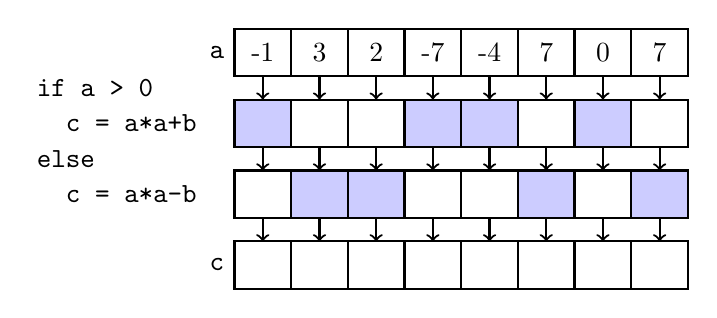
\begin{tikzpicture}[scale=0.6,thick]
    \foreach \x/\num in {0/-1, 1.2/3, 2.4/2, 3.6/-7, 4.8/-4, 6/7, 7.2/0, 8.4/7}
    {
        \draw (\x, 0) node {\num} +(-.6, -.5) rectangle ++(.6, .5);
        \ifnum \num > 0
            \draw (\x, -1.5) +(-.6, -.5) rectangle ++(.6, .5);
            \draw[fill=blue!20] (\x, -3) +(-.6, -.5) rectangle ++(.6, .5);
        \else
            \draw[fill=blue!20] (\x, -1.5) +(-.6, -.5) rectangle ++(.6, .5);
            \draw (\x, -3) +(-.6, -.5) rectangle ++(.6, .5);
        \fi
        \draw (\x, -4.5) +(-.6, -.5) rectangle ++(.6, .5);
        \draw[->] (\x, -0.5) -- (\x, -1);
        \draw[->] (\x, -2) -- (\x, -2.5);
        \draw[->] (\x, -3.5) -- (\x, -4);
    }
    \node[anchor=east] at (-0.6, 0)    {\texttt{a}};
    \node[anchor=west] at (-5, -0.75)  {\texttt{if a > 0}};
    \node[anchor=west] at (-5, -1.5)   {\texttt{~~c = a*a+b}};
    \node[anchor=west] at (-5, -2.25)  {\texttt{else}};
    \node[anchor=west] at (-5, -3)     {\texttt{~~c = a*a-b}};
    \node[anchor=east] at (-0.6, -4.5) {\texttt{c}};
\end{tikzpicture}
\caption{Branch divergence in parallel execution.
    Shaded boxes indicate idle threads. Adapted from~\cite{Hijma2023}.
}\label{fig:branching}
\end{figure}

A workgroup can also have shared memory,
in addition to the global memory buffers that are accessible by all workgroups
of a shader invocation.
Whenever data is shared between threads,
it is important to understand how much synchronization is required,
because the memory model actually makes very few guarantees about the ordering
of memory operations.
Workgroups can be executed with any amount of parallelization and in any order.
Even synchronization within a workgroup is not guaranteed,
but can be enforced with special synchronization barriers.
These barriers have to be passed by all threads of a workgroup simultaneously,
guaranteeing the order of memory operations between threads~\cite{wgsl_spec}.

Many algorithms would however benefit greatly from the ability for
synchroniziation between workgroups.
Newer GPUs do include architectural changes that allow for some amount of
inter-workgroup synchronization~\cite{Hijma2023}.
However, this feature is not available in WebGPU due to a limitation within
Metal, which also prohibits using it on other platforms in the spirit of
portability~\cite{Levien2021}.
The topic of synchronization is further discussed in
Section~\ref{subsec:defend_shader} in the context of this work.
